\mychapter{It never rains, but it pours}

\section{Rules}

\subsection{Materials}
To play this game you need:
\begin{itemize}
    \item at least two players
    \item a sheet of paper
    \item at least one pen or pencil (in the following it is assumed that there
        are two: one blue and one black)
    \item player tokens, one for each player
    \item a pair of dice (this document assumes two six-sided dice, but any
        number of sides can work, they don't even have to have the same number
        of sides), peferably of different colours so that they can be told
        apart
\end{itemize}

\subsection{Preparation}
Collect the necessary materials and create a board following the directions
in~\ref{ch:board}.

Each player rolls the pair of dice and places their player token in the
position indicated.

The player who rolled the highest sum takes the first turn, the play then
proceeds in clockwise order (unless all players are either mathematicians or
physicists, in which case play proceeds in anti-clockwise order).

\paragraph{Example:}
\begin{itemize}
    \item \Kim{}, \Rufus{} and \Xing{} are playing. They have two six-sided
        dice and decide to use the example board from the back of the rule
        booklet.
    \item They decide to use the red die for the first coordinate and the
        black die for the second.
    \item They each roll the dice in turn and place their player tokens:
        \begin{itemize}
            \item \Kim{} rolls \rdie3 \die6 and places a token on 3,~6.
            \item \Rufus{} rolls \rdie4 \die2 and places a token on 4,~2.
            \item \Xing{} rolls \rdie3 \die4 and places a token on 3,~4.
        \end{itemize}
    \item Since \Kim{} rolled the highest sum, she starts. Since \Rufus{} is a
        biologist, play then proceeds in a clockwise manner.
\end{itemize}
The resulting positions can be seen in Figure~\ref{fig:start}.

\begin{figure}[t]
    \centering
    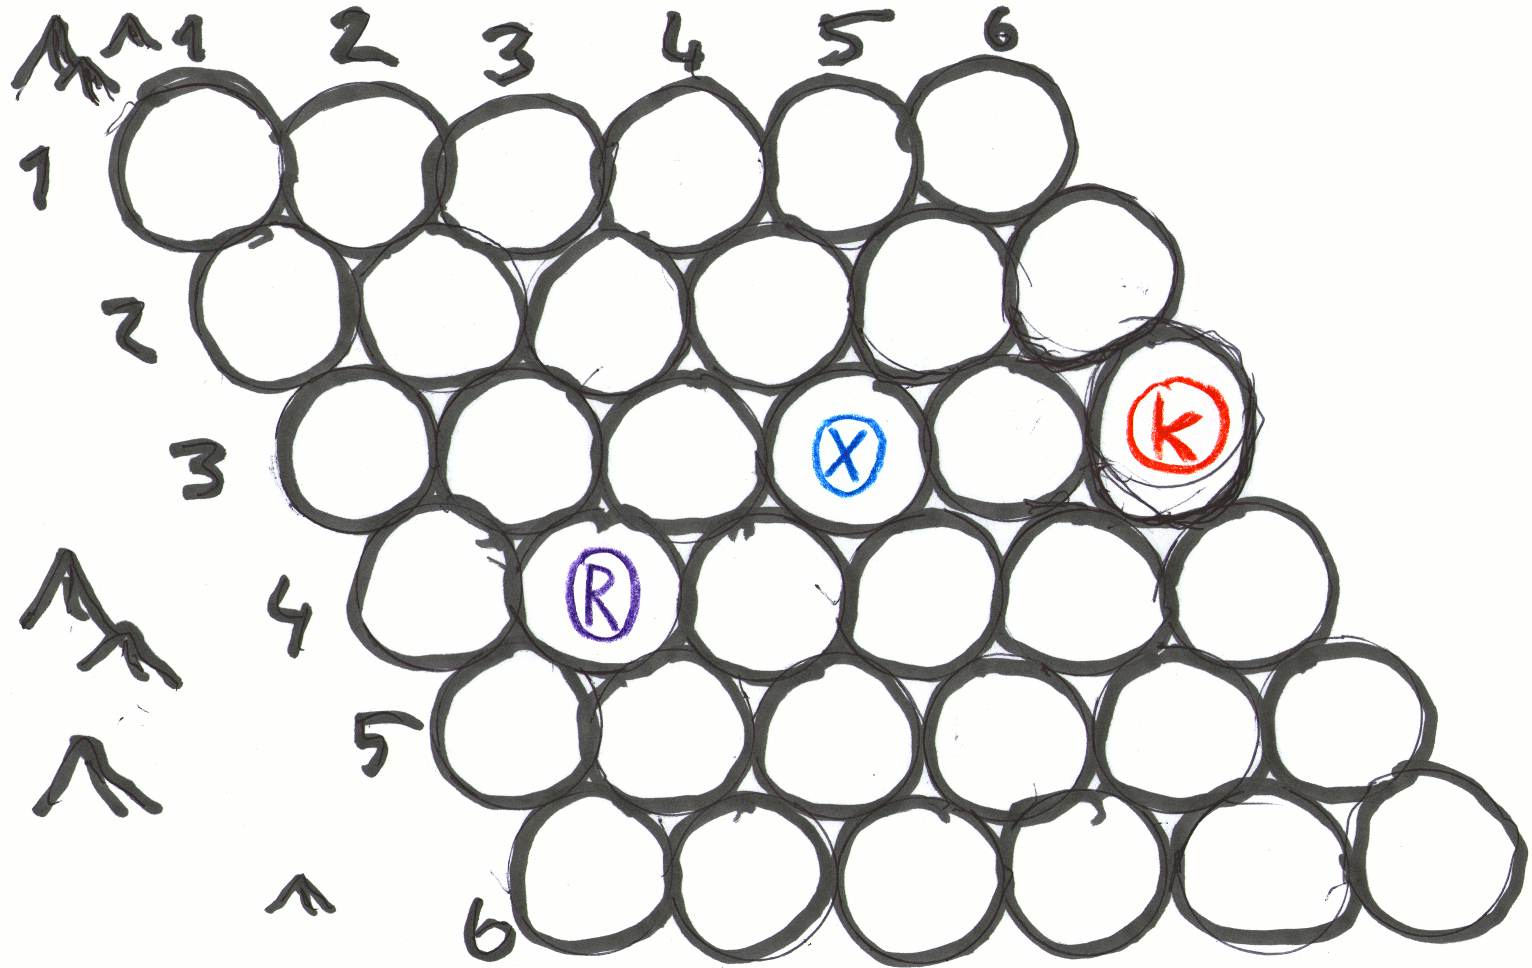
\includegraphics[width=0.95\textwidth]{board_start}
    \caption{\textbf{Setup:} Starting positions for \Kim{}, \Rufus{} and
        \Xing{}}
    \label{fig:start}
\end{figure}

\subsection{Objective}
The objective of the game is to stay on the board for as long as possible,
avoiding to get stuck or be flushed away, while trying to out-manoeuvre the
other players.

\subsection{The player turn}
Each player in turn goes through the following steps:
\begin{enumerate}
    \item roll the dice
    \item take action: move, build or push
    \item resolve rain and flash flood
\end{enumerate}

\subsubsection{Roll dice}
Roll both dice, but make sure to keep track of which die represent which
coordinate. For this purpose, it helps to have different coloured dice.

\subsubsection{Take action}
\paragraph{Move}
Move your token to an adjacent space \emph{without water}.

If you start your turn in a space that is under water, this is the only action
you are allowed to take.

\begin{SCfigure}
    \centering
    \caption{\textbf{Moving:} Since she is pretty far down-stream, \Kim{} uses
        her action to move up-stream. She can move to any of the indicated
        positions.}
    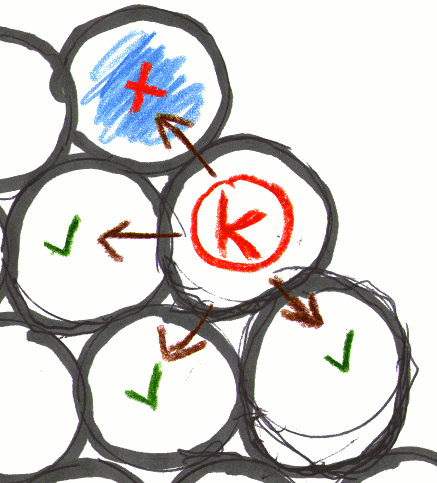
\includegraphics[width=0.38\textwidth]{move_example}
    \label{fig:move_example}
\end{SCfigure}

\paragraph{Build}
If you start your turn in a dry space without a channel, you may build a
channel there. Draw a line through the space between any two neighbouring
spaces on the board. If any of the connected spaces already has a channel,
connect these to the new channel - this is the only way a channel can get
forks. A channel may connect a space on the board with the outside of the
board, but only only if the space outside the board is down-stream. A channel
may, however, connect two up-stream spaces, possibly allowing a flash flood to
flow up-stream (see~\ref{sec:flood}).

\begin{SCfigure}
    \centering
    \caption{\textbf{Building:} The water up-stream of \Rufus{} is making him
        nervous. \Rufus{} decides to build a channel and can do so between any
        two of the indicated neighouring spaces, including ``space'' outside
        the board down-stream.}
    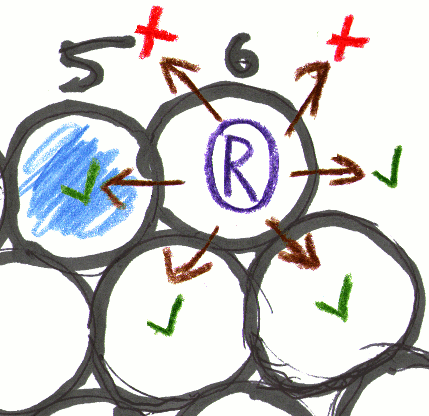
\includegraphics[width=0.38\textwidth]{channels_example}
    \label{fig:channels_example}
\end{SCfigure}

\paragraph{Push}
If you start your turn in the same space as another player, you may choose as
your action to push that player to any adjacent space. The new space doesn't
have to be empty, it may have both water and/or other players. You may not,
however push a player off of the board.

\begin{SCfigure}
    \centering
    \caption{\textbf{Pushing:} Since \Xing{} started his turn in the same space
        as \Kim{}, \Xing{} has the option to push her to any of the indicated
        spaces as his action. \Xing{} may not push \Kim{} out of the board, but
        may push \Kim{} into a space where there might soon be flash flood!}
    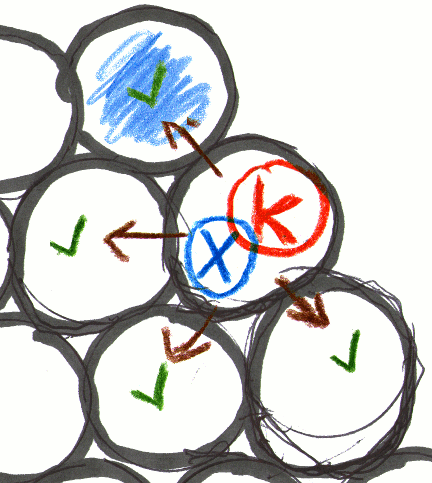
\includegraphics[width=0.38\textwidth]{push_example}
    \label{fig:push_example}
\end{SCfigure}


\subsubsection{Resolve rain and flash floods}
\paragraph{Rain}
Find the space indicated by the dice roll. If it is dry or has a channel, then
mark it to show that it is now under water. If it is already under water or if
there is a channel, then a flash flood occurs.

\paragraph{Flash flood}
\label{sec:flood}
If rain falls in a space that already has water or has a channel, a flash flood
occurs and the water flows to an adjacent space. If that space already has
water or the flash flood flows into a channel, that space to is flooded and
this step is repeated.

Floods happen according to the following rules:
\begin{itemize}
    \item A flash flood may only flow into or out of an area with a channel
        along the channel. \textbf{Exception:} If there are no other legal
        moves, or the flash flood would otherwise go around in a loop, the
        flash flood may break the channel walls. The channels in areas thus
        broken into and/or out of are destroyed, the areas marked as under
        water, and the flash flood stops.
    \item The flash flood may only move up-stream if it cannot move
        horisontally or down-stream.
    \item The flash flood stops either when the water reaches a dry space or
        flows off the board.
    \item If the flash flood flows through a space with a player token, either
        through a channel or because the area is already under water, the
        player is washed along with the flash flood until it stops or flows off
        the board.
\end{itemize}
Within these limits, it is up to the active player to decide where the flash
flood flows.

\begin{figure}[t]
    \centering
    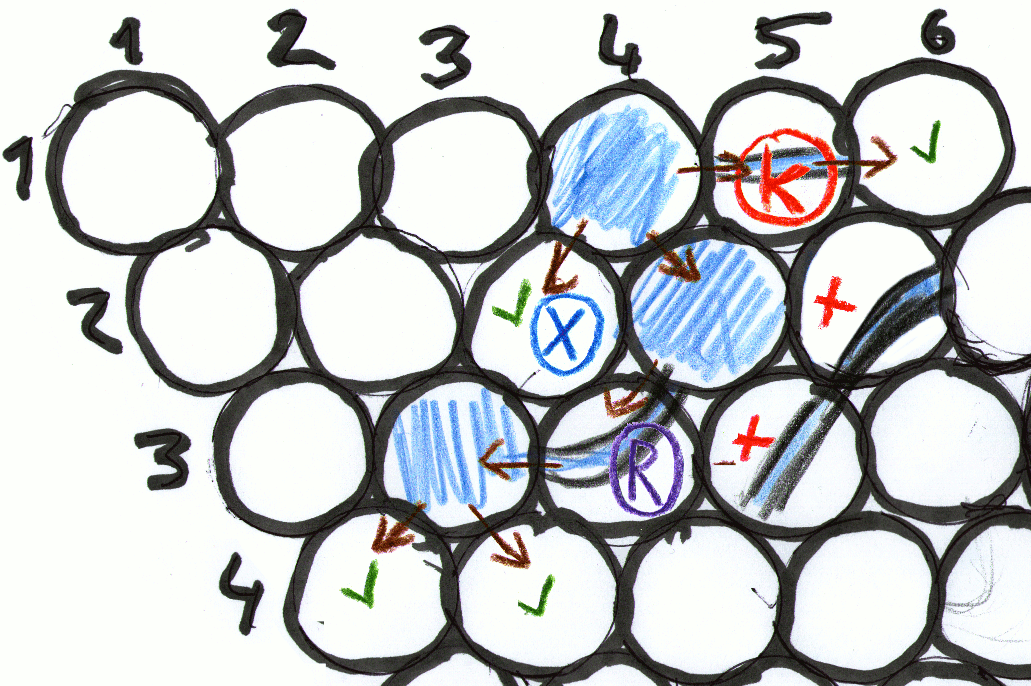
\includegraphics[width=0.89\textwidth]{flash_flood_example}
    \caption{\textbf{Flash flood:} The current player has rolled \rdie1 \die4
        causing a flash flood. The flood can either be diverted to \Xing{}'s
        position at 2,~3, or into the channel where \Kim{} is standing,
        sweeping her with it to 1,~6, or finally by the longer route through
        \Rufus{}'s location, sweeping him away to either 4,~1 or 4,~2. There is
        no risk of anyone being swept off of the board at this point, but
        whatever happens, someone is getting wet!}
    \label{fig:flash_flood_example}
\end{figure}

\subsection{Winning and losing}
There are two ways for a player to be ousted from the game:
\begin{itemize}
    \item If when their turn comes, a player has no legal moves, they are out
        of the game. Remove their token.
    \item If a player token is washed along with a flash flood and it thereby
        ends up outside the board, that player is out of the game.
\end{itemize}
The last player to remain on the board is the winner.


\section{Summary}
\begin{itemize}
    \item Roll dice to determine player starting spaces, highest sum starts
    \item Each player in turn goes through the following steps:
    \begin{enumerate}
        \item roll the dice
        \item take action: move, build or push
        \item resolve rain and flash floods
    \end{enumerate}
    \item Play proceeds until there is only one player left on the board
        -- this player is the winner.
\end{itemize}


\newpage

\section{Variants}
Here are a few variant rules that give rise to different kinds of choices.
Most of them are compatible and can be combined. Neither the base game nor the
variants below have been thoroughly tested. Feedback is much appreciated!

\subsection{Indistinct dice}
To give the players more choice, the player decides in which order to interpret
the dice, for the prupose of placing rain.

\subsection{No foresight}
Swap the order of steps 1. and 2. in the turn sequence, so that the action is
taken before the player knows where it will rain.

\subsection{More actions}
Let each player take two actions each turn instead of just one. If the player
starts in water, the first action still has to be to move.

\subsection{Squares}
Use squares rather than hexagons for the board. Squares are more boring than
hexagons, but if you want to play with dice with many more sides, it will make
the board construction much simpler. Players and floods move in any of the
eight directions, following the normal rules, with up-stream and down-stream
opposing corners of the board.

\subsection{Teams}
Divide into several teams of two or more players to play a semi-cooperative
version, where the team wins together if one of their players is the last one
left on the board. Make sure to be seated so that the turn order is distributed
fairly between all teams.

\subsection{Live action}
Follow the basic rules with any of the variants above, but make the board large
enough, that you can use yourselves as tokens. Probably best played on the
beach or similar, where you can draw the board and channels in the sand.
